\chapter[Learning Occluded Branch Depth Maps in Forest Environments]{Learning Occluded Branch Depth Maps in Forest Environments using RGB-D Images}
\label{ch:OBR}

% % \newcommand{\figurevspaceabove}{-0.6cm}
% % \newcommand{\figurevspacebelow}{-0.3cm}
% \newcommand{\figurevspaceabove}{-0.5cm}
% % \newcommand{\figurevspaceabove}{0cm}
% \newcommand{\figurevspacebelow}{-0.5cm}
% % \newcommand{\figurevspacebelow}{0cm}
\newcommand{\figurevspaceabove}{0cm}
\newcommand{\figurevspacebelow}{0cm}


\author{
Christian~Geckeler,
Emanuele~Aucone,
Yannick~Schnider,
Andri~Simeon,\\
Jan-Philipp~von~Bassewitz,
Yunying~Zhu,
and Stefano~Mintchev% <-this % stops a space
\thanks{This work was supported by the Swiss National Science Foundation through the Eccellenza Grant number 186865.}% <-this % stops a space
\thanks{The authors are with the Environmental Robotics Laboratory, Dept. of Environmental Systems Science, ETH Zurich, 8092 Zurich, Switzerland and with the Swiss Federal Institute for Forest, Snow and Landscape Research (WSL), 8903 Birmensdorf, Switzerland. (e-mail: \{cgeckeler, eaucone, yannicks, ansimeon, vbjan, yunzhu, smintchev\}@ethz.ch)}%
}

\begin{abstract}
Covering over a third of all terrestrial land area, forests are crucial environments; as ecosystems, for farming, and for human leisure. However, they are challenging to access for environmental monitoring, for agricultural uses, and for search and rescue applications. To enter, aerial robots need to fly through dense vegetation, where foliage can be pushed aside, but occluded branches pose critical obstacles. Therefore, we propose pixel-wise depth regression of occluded branches using three different U-Net inspired architectures. Given \mbox{RGB-D} input of trees with partially occluded branches, the models estimate depth values of only the wooden parts of the tree. A large photorealistic simulation dataset comprising around 44K images of nine different tree species is generated, on which the models are trained. Extensive evaluation and analysis of the models on this dataset is shown. To improve network generalization to real-world data, different data augmentation and transformation techniques are performed. The approaches are then also successfully demonstrated on real-world data of broadleaf trees from Swiss temperate forests and a tropical Masoala Rainforest. This work showcases the previously unexplored task of frame-by-frame pixel-based occluded branch depth reconstruction to facilitate robot traversal of forest environments.
All models, code, and data are available online. \cite{Geckeler2023OBRSupplementary}\footnote{All models, code and data are available online: \href{https://doi.org/10.3929/ethz-b-000634419}{https://doi.org/10.3929/ethz-b-000634419} \cite{Geckeler2023OBRSupplementary}}
\end{abstract}

% % Keywords appear just beneath the abstract. Use only for final RAL version. 
% \begin{IEEEkeywords}
% Deep Learning for Visual Perception; Robotics and Automation in Agriculture and Forestry; RGB-D Perception
% \end{IEEEkeywords}

\section{Introduction}
Forests represent an integral part of Earth's biosphere, covering over a third of all terrestrial land area \cite{FAO2020a}, supporting more than half of the world's vertebrate species \cite{Pillay2022} as well as providing essential ecosystem services and climate regulation~\cite{Brockerhoff2017}. %, Nakamura2017}.
Additionally, 43\% of all agricultural land globally has at least 10\% tree cover \cite{Zomer2016}. Dozens of meters tall and often situated in remote locations, they are challenging to access and survey.

%Loquercio2021, Hedgehog
These circumstances present a natural opportunity for autonomous and highly agile micro aerial vehicles (MAVs), which are beginning to demonstrate flight above and below tree canopies in forests with sparse vegetation~\cite{Zhou2022, Liu2022}. MAVs are also being utilized for environmental tasks such as sample collection from above the treetops \cite{Charron2020}, or sensor placement and environmental monitoring in the outermost canopy regions~\cite{Geckeler2022a, Aucone2023a, Hamaza}.

Besides environmental monitoring, MAVs are also demonstrating increased use in agriculture, such as for sensing and detection in orchards \cite{Zhang2021}, or fruit harvest \cite{Tevel}, as well as for search and rescue operations in forest environments \cite{Schedl2021}. 
%Giusti2016

\begin{figure}[!t]
\centering
\includegraphics[width=1\columnwidth]{chapters/papers/OBR/figures/fig-1-overview/fig-1-overview-v03.pdf}
\vspace{\figurevspaceabove}
\caption{(A) Simulation RGB tree image (left) and predicted depth point cloud only for branches (right). (B) Predicted pixel-wise depth values only for branches, on real images from trees from a Masoala Rainforest (colorbar in meters).
%Predicting pixel-wise depth values only for branches, on real images from trees from a Masoala Rainforest.
}
\label{fig-1-overview}
% \vspace{\figurevspacebelow}
\vspace{-0.6cm}
\end{figure}
The challenge of navigating through cluttered and dense foliage remains a significant hurdle for MAVs, rendering tree canopies largely inaccessible. Recent developments have shown that since MAVs can push aside compliant obstacles \cite{Aucone2023}, twigs and leaves would pose little threat to MAVs with shielded propellers \cite{Mulgaonkar2018b},
% DePetris2022}, % Kornatowski2017}, % removed for space
%deAzambuja2022WhenExoskeletons,
but colliding with thick branches and the trunk might destabilize the drone and result in a fatal crash. Therefore, a perception system to detect the wooden parts of the tree - the branches and the trunk - is necessary. Partially or fully occluded branches pose a major challenge, especially in forest environments. This prevents the application of classic computer vision approaches based on shape, feature, or color detection. 
% In \cite{Andresen2022} the authors demonstrate a haptic system to detect branches occluded by leaves, but only stiff branches can be detected whereas softer ones are confused with foliage.
Artificial neural networks have demonstrated much promise in generative assistance for visual perception in challenging environments, including  Generative Adversarial Networks (GANs) \cite{Islam2020}.
%<TODO mabye cite another GAN/self-supervised for image enhancement

To address these challenges, this letter proposes a neural network-based system to predict the pixel-wise depth values only of the wooden parts of the tree (see Figure~\ref{fig-1-overview}), given a single RGB-D image (RGB and depth) of trees with partially occluded branches.
Utilizing a photorealistic simulator, a large RGB-D dataset of different tree species with and without leaves is generated. The synthetic data is then used to train U-Net inspired encoder-decoder networks. To improve network
generalization to real-world data, different data augmentation and transformation techniques are performed. Finally, to validate the approach, the feasibility of the outputs is shown on real data from two discrete biomes. 

The main contributions of this work are as follows:
\begin{itemize}
    \item Generation of a dataset with around 44K RGB-D images of nine different species of photorealistic simulated trees, with and without leaves; transformed and augmented for real-world domain adaptation (training and groundtruth, datasets available online \cite{Geckeler2023OBRSupplementary}).
    \item Training and extensive quantitative evaluation of three different U-Net\cite{Weng2015a}-inspired architectures on the previously unexplored topic of predicting pixel-wise depth of occluded tree structures from a single frame using simulated data (code available online \cite{Geckeler2023OBRSupplementary}).
    \item Qualitative evaluation of the networks on real-world data from trees from Swiss temperate forests and a rainforest, demonstrating the real-world utility of the approach (data captures available online \cite{Geckeler2023OBRSupplementary}).
\end{itemize}  

\section{Related Works}
% also include fast underwater image enhancement \cite{Islam2020}, some insight about training in simulation or utility from the application

% The research areas of RGB-D semantic segmentation and monocular depth estimation offer insights into the problem of predicting depth values of occluded branches. The former covers RGB-D input data encoding strategies, while the latter demonstrates how the models can be supervised. 
% monocular depth estimation hile the latter demonstrates how the models can be supervised. 

The depth estimation of occluded natural structures is mostly unexplored. Recently, an offline heuristic-based approach for extracting occluded tree skeletons in orchards was presented in \cite{Kim2023}. First, visible branches are extracted via RGB instance segmentation, which are then "extended" in the longitudinal branch direction, resulting in a 3D likelihood map of potential branch locations. Using images from multiple viewpoints, the final tree skeleton is then extracted through consolidating the line segments, smoothing them, and connecting them through minimum cost path search. While this approach produces feasible results on simulated trees, it requires parts of branches to be visible in the instance segmentation step. This, along with the heuristic assumption that branches grow straight, fundamentally limits the approach to comparatively simple tree topologies with partially visible branches. Indeed, the qualitative results on the real apple orchard trees show that often branches are truncated due to heavy foliage occlusion, or missed entirely.

While not dealing with occluded branches, in \cite{Kierdorf2022}, a GAN was used to predict probable grayscale masks of occluded grapes. The networks were trained on masked grayscale images of manually exfoliated grapes which were then synthetically occluded. This represents a comparatively simple scenario since the occluded target grape clusters are identifiable in the images, and follow predictable grouping patterns. In contrast, tree branches in the wild can be more densely occluded, and branch locations cannot easily been inferred based on leaf clustering patterns, since global visual cues about the tree structure may not be available from short distances. 

The less complex problem, since the output is a 2D mask, of semantic segmentation on partially occluded branches is covered in \cite{Chen2021d}, where manually annotated RGB-D images of apple trees were used to train a conditional GAN, a U-Net, and a Convolutional Neural Network (CNN). The even simpler case of semantic segmentation of tree-like vegetation from RGB-D input, neglecting occlusions, is investigated in \cite{TejaswiDigumarti2019}.
In existing literature, most approaches are limited to well-structured and visually similar situations, such as apple trees or vineyards, and do not address dense occlusions from variable camera angles with changing depth scales or out-of-distribution species. Most importantly, all of these approaches lack 3D depth information in the output, which is critical for robot navigation.

When training networks to regress pixel-wise depth values of occluded branches, inspiration can be taken from monocular depth estimation. The problem of inferring depth information from a single RGB image in a supervised setting can also be seen as a pixel-wise regression problem. A CNN was first used in \cite{eigen2014firstNNdepth_map_pred} to approach this regression task, with different loss functions proposed in the literature thereafter. While the $\mathcal{L}_2$-loss represents a common loss function for regression, model-specific loss functions were designed in \cite{eigen2015specific_loss_d_esti}, 
%%eigen2014firstNNdepth_map_pred
and  \cite{laina2016resnet_for_d_esti} reports better results using a deep fully convolutional residual network and training on the reverse Huber loss.
% There is a wide range of Deep Learning approaches to monocular depth estimation using Convolutional Neural Networks (CNNs) \cite{eigen2014firstNNdepth_map_pred}, Recurrent Neural Networks (RNNs)\cite{wang2019RNN_for_d_estimation} and Generative Adversarial Networks (GANs) \cite{chakravarty2019GAN_for_d_estimation}. 
% In the supervised setting, the problem of monocular depth estimation can be seen as a pixel-wise regression problem. 
% A CNN was first used in \cite{eigen2014firstNNdepth_map_pred} to perform this regression task. Different loss functions have been proposed in the literature thereafter. $\mathcal{L}_2$-loss and other common regression loss functions yield themselves as obvious options. Specific loss functions for the models were designed in \cite{eigen2014firstNNdepth_map_pred, eigen2015specific_loss_d_esti}. In line with other deep learning research efforts, \cite{laina2016resnet_for_d_esti} reports better results using a deeper fully convolutional residual network and training on the reverse Huber loss.

To regress pixel-wise depth values based on RGB-D input, the color and depth channels must be properly encoded. Although the problem formulation is slightly different, previous literature on semantic segmentation with RGB-D inputs offers insights into RGB-D input encoding strategies.
%improving_seg_with_RGBD removed for space
Additional depth information for RGB images has shown to increase segmentation performance \cite{Depth-awareCNN}. However, it is challenging to fuse the color and depth information in the encoder, due to their different modalities. Naively concatenating the depth information as an additional channel to the RGB channels (\textit{early fusion}) usually results in worse performance on segmentation tasks \cite{wang2021dl_rgb_seg_review} than the following more evolved strategies.
%
\textit{Late fusion} approaches treat color and depth data in isolation to fuse their respective feature representations at a later stage in the network \cite{xing2019coupling}. Distinct processes extract the relevant segmentation features from each modality separately, which are later combined into a single representation. This fusion can happen before the network decoder \cite{jiang2018rednet} or even at the output layer \cite{TejaswiDigumarti2019}. In \cite{gupta2014HHA_encoding}, the depth input is encoded as an HHA image (horizontal disparity, height above the ground, and the angle of the pixel’s local surface normal with the gravity direction) and then concatenated with a segmentation mask predicted by an RGB segmentation model. The resulting tensor is then passed through a final network to refine the previously predicted segmentation mask.

An alternative to the introduced late and early fusion approaches is to fuse the two modalities at each decoding step (\textit{decoder fusion}). In \cite{Depth-awareCNN} the authors show that fusing at different decoding stages indeed improves segmentation performance. In contrast, depth and RGB feature representations are fused at each encoder stage in \cite{Seichter2020ESANet, jiang2018rednet} (\textit{encoder fusion}). This approach only requires a single decoder, which reduces its computational complexity. The authors of \cite{Seichter2020ESANet} propose a lightweight architecture called ESANet, following the encoder fusion strategy.

%-----------------------------------------------------------------------------

% To the best of the authors' knowledge the task of pixel-wise depth regression based on RGB-D input has not yet been investigated.
The task of pixel-wise depth regression based on RGB-D input has not been extensively investigated. However, for robot navigation depth information is essential - the closer a branch is, the more immediate the threat of a potential collision. Additionally, the information about occluded obstacles can be utilized for obstacle avoidance and path planning. 

\section{Methodology}
% - first describe different network architectures, how the simulation dateset is created, and how the data was augmented for the sim-to-real transfer
In this section, we describe the sensor choice, the network architectures, the dataset generation, the training procedure, and the domain adaptation techniques eventually used for depth predictions based on real-world input data. 
This work focuses on deciduous trees, since the problem is more challenging, with larger leaves presenting more opportunities for occlusions. Additionally, the wooden part of the branches of coniferous trees can be more easily inferred, since each needle is directly attached to a branch, giving more information about the location and shape of the branch.

\subsection{Sensor Choice}
Depth cameras present a mature, relatively cheap, and off-the-shelf solution for acquiring color and depth information from a scene.
\mbox{RGB-D} input has also been demonstrated to be sufficient for robot localization and navigation: below the canopy, high speed learning-based end-to-end flights using only depth images as input \cite{Loquercio2021}, as well as depth and LiDAR input integrated into more traditional perception and mapping pipelines \cite{Zhou2022, Liu2022} have been demonstrated. % (Zhou2022 depth camera justification \cite{}
While LiDAR presents an increasingly popular choice of perception sensor for aerial robots \cite{DePetris2022, Liu2022}, the size, weight, price, and large minimum detection range make it ill-suited for small MAVs used to explore the inside of close-range and dense forest canopies. RGB-D sensors do not suffer from these drawbacks and are therefore chosen for this work.  

\begin{figure}[!t]
\centering
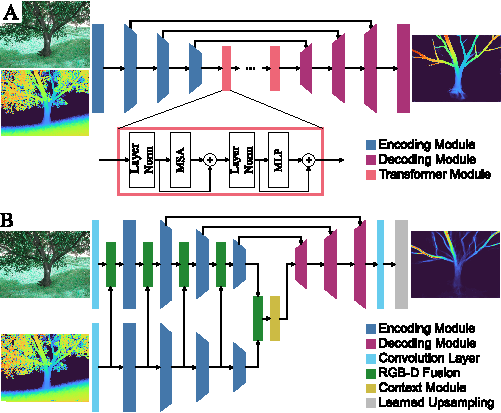
\includegraphics[width=1\columnwidth]{chapters/papers/OBR/figures/fig-2-networks/fig-2-networks-v02.pdf}
\vspace{\figurevspaceabove}
% \vspace{1cm}
\caption{Network architectures: (A) TransUNet \cite{Chen2021c}, and (B) ESANet \cite{Seichter2021}.}
\label{fig-2-networks}
\vspace{\figurevspacebelow}
\end{figure}

\subsection{Network Architectures}
\label{sec:models}
All models presented in this section encode the pixel-wise feature channels to a low dimensional manifold, then decode the compressed information to obtain a pixel-wise output image. 
To compare different models, a baseline model (\textit{Baseline}) was designed: an established U-Net style architecture \cite{ronneberger2015u} performs binary segmentation which is in turn used to mask the input depth data. The target segmentation mask has two classes: tree skeleton pixels (wooden parts) and all remaining pixels as the second class. The early fusion approach was used to concatenate the normalized depth values to the RGB color channels as input to the segmentation U-Net. The final baseline model outputs depth maps containing values only for pixels of the trunk or branches, either visible or occluded. This approach requires intermediate processing steps and is unable to deal with occlusions, nonetheless it presents a meaningful baseline, without loss of generality.

Our first model (U-Net) is the U-Net architecture expanded to perform regression, providing an end-to-end extension of the baseline model, which is able to handle occlusions.
While the network encoder remains the same, using early fusion, the logistic activation in the last decoding layer is removed and a single output channel is used.

Similarly, the second model (TransUNet) \cite{Chen2021c} is based on the U-Net architecture with the addition of transformer layers bridging the encoder and decoder module for enhanced feature extraction with global context. The architecture can be seen in Figure~\ref{fig-2-networks}A. Firstly, a feature extractor in the form of the first four layers of a pre-trained U-Net is utilized. Then, a patch and positional embedding, followed by 12 transformer layers, refine the previously obtained features. Finally, the decoder tightly follows the implementation of the U-Net adjusted for regression. The TransUNet also exploits the early fusion approach for the RGB-D input.

In contrast to all the previous models, this last model (ESANet) utilizes the late fusion approach for incorporating the depth information. A simplified diagram of the model is shown in Figure~\ref{fig-2-networks}B.
The ESANet is based on an RGB-D semantic segmentation architecture \cite{Seichter2020ESANet}, which fuses color and depth at different stages of the encoder. The decoder is modified for depth estimation by enforcing a single output channel with sigmoid activation function, which scales to the minimum and maximum depth (0m and 10m).

\subsection{Data Generation}
Generating a real-world dataset for model training is infeasible, since exactly the same RGB and depth image of the scene with and without leaves is required. Manually removing foliage disturbs the branches and alters their resting position due to the changed weight distribution. Waiting for seasonal abscission also results in changes and movement of the branches due to the tree growing and changing over such a long time span. Similarly, manually annotating and removing leaves from the 3D depth data is not feasible, since the depth would have to be estimated for each occluded pixel, which would be as challenging as the actual task.

Therefore, a photo-realistic simulator is used to generate the data (Figure~\ref{fig-3-sim-training}-IA, -IB), which greatly simplifies the data collection process since foliage can easily be removed from the tree model without any changes to branch position. Data generation was semi-automated, with grids of 9 to 13 trees of seven species (Elm, Maple, Amur Cork, Black Alder, London Plane, Weeping Beech, and American Sycamore) randomly and procedurally generated using SpeedTree$^\text{\textregistered}$ \cite{SpeedTree}. To generate images, the tree models were loaded into Unreal Engine 4 \cite{Unreal4.27}, where the UnrealCV plugin \cite{UnrealCV} was used to simulate an RGB-D sensor for automated data collection. For more realistic sensor emulation, for instance the Intel Realsense D435 series, simulated sensor noise was added \cite{Ahn2019AnalysisRobots} and the depth was cut off at ten meters. A separate ground-truth level was created where the foliage had been removed from the trees. 

Five different helical trajectories, orbiting each tree to simulate drone flight, were used to capture image data from different views - 500 images were captured per tree. Several additional processing steps are executed to more accurately emulate the reduced quality of a real depth camera, see Section~\ref{subsec:domain_adaptation} for details. 
% \vspace{-6em}
\begin{figure}[!t]
\centering
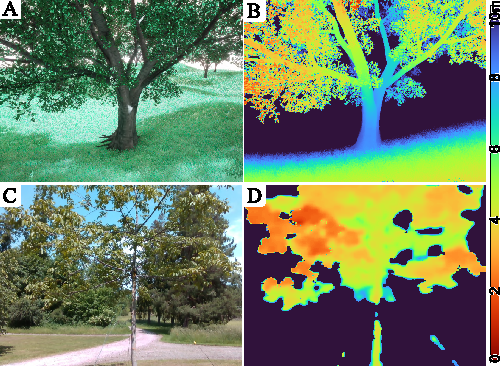
\includegraphics[width=1\columnwidth]{chapters/papers/OBR/figures/fig-3-sim-training/fig-3-sim-training-v02.pdf}
\vspace{\figurevspaceabove}
\caption{RGB (A-I) and depth (B-I) data obtained in the Unreal Engine simulation, and real RGB (A-II) and depth (B-II) data captured with the Intel Realsense D435 depth sensor. Colorbar on the right shows depth scale in meters.}
\label{fig-3-sim-training}
\vspace{\figurevspacebelow}
\end{figure}

\subsection{Training}
\label{subsec:training}
The simulated dataset is evenly divided into training, validation, and test sets across tree species, with eight to nine trees from each species for training (30K images), two trees for validating, and two trees for testing (7K images each). The validation and test set comprise images from previously unseen trees, although different trees of the same species are present in the training data. Additionally, two different species; Walnut and Shagbark Hickory, were held out entirely during training to evaluate the generalization abilities of the proposed network architectures.

{\small
\begin{align}
\label{eq:MSE}
\vspace{\figurevspaceabove}
\mathit{MSE}=\frac{1}{mn} \sum_{i=1}^m \sum_{j=1}^n (p_{ij}-t_{ij})^2\\[2ex]
\begin{array}{@{} l >{$}l<{$} @{}}
m      & number of rows in image\\ \nonumber
n      & number of columns in image\\ \nonumber
p_{ij} & predicted depth value at pixel\\ \nonumber
t_{ij} & ground truth depth value at pixel \nonumber
\end{array} \\ \nonumber
\vspace{-0.6cm}
\end{align}
}%
% \vspace{-0.2cm}

% Several loss functions were evaluated for network training. They can be grouped into loss functions for binary segmentation (including cross entropy, dice loss \cite{diceLoss}, focal loss \cite{focalLoss}, and Tversky loss \cite{tverskyLoss}), and loss functions for regression (including mean square error (MSE) as in Equation~\ref{eq:MSE}, root mean square error (RMSE), logarithmic RMSE (LogRMSE), smooth L1 loss, and adaptive smooth L1 loss). In Equation~\ref{eq:MSE} $m$ is the number of rows in the image, $n$ is the number of columns, $p_{ij}$ is the predicted depth value at the pixel, and $t_{ij}$ is the ground truth depth value at the pixel.

% Several loss functions were evaluated for network training. They can be grouped into loss functions for binary segmentation (including cross entropy, dice loss, focal loss, and Tversky loss), and loss functions for regression (including mean square error (MSE) as in Equation~\ref{eq:MSE}, root mean square error (RMSE), logarithmic RMSE (LogRMSE), smooth L1 loss (SmL1), and adaptive smooth L1 loss (AdSmL1)). 
Several loss functions were evaluated for network training. They can be grouped into loss functions for binary segmentation (including cross entropy, dice loss, focal loss, and Tversky loss), and loss functions for regression (including mean square error (MSE) as in Equation~\ref{eq:MSE}, root mean square error (RMSE), logarithmic RMSE (LogRMSE), smooth L1 loss (SmL1), and adaptive smooth L1 loss (AdSmL1)). 

% {\small
% \begin{align}
% \label{eq:MSE}
% \mathit{MSE}&=\frac{1}{mn} \sum_{i=1}^m \sum_{j=1}^n (p_{ij}-t_{ij})^2 \phantom{iiiiiiii}\\[2ex]
% \label{eq:RMSE}
% \mathit{RMSE}&=\sqrt{\frac{1}{mn} \sum_{i=1}^m \sum_{j=1}^n (p_{ij}-t_{ij})^2} \phantom{iiiiiiii}\\[2ex]
% \label{eq:LogRMSE}
% \mathit{LogRMSE}&=\sqrt{\frac{1}{mn}\sum_{i=1}^m\sum_{j=1}^n(log(p_{ij}+1)-log(t_{ij}+1))^2}\\[2ex]
% \label{eq:AbsRelErr}
% \mathit{AbsRelErr} &= \frac{1}{mn} \sum_{i=1}^m \sum_{j=1}^n \frac{\lvert p_{ij}-t_{ij} \rvert}{t_ij} \phantom{iiiiiiii}\\[2ex]
% \label{eq:SqRelErr}
% \mathit{SqRelErr} &= \frac{1}{mn} \sum_{i=1}^m \sum_{j=1}^n \frac{( p_{ij}-t_{ij} ) ^2}{t_ij} \phantom{iiiiiiii}
% % \mathit{MSE}=\frac{1}{mn} \sum_{i=1}^m \sum_{j=1}^n (p_{ij}-t_{ij})^2 \phantom{iiiiiiii}\\[2ex]
% % \begin{array}{@{} l >{$}l<{$} @{}}
% % m      & number of rows in image\\ \nonumber
% % n      & number of columns in image\\ \nonumber
% % p_{ij} & predicted depth value at pixel\\ \nonumber
% % t_{ij} & ground truth depth value at pixel \nonumber
% % \end{array} \\ \nonumber
% \end{align}
% }%


% The following evaluation metrics as proposed and defined in \cite{eigen2014firstNNdepth_map_pred} are used to compare the performance: MSE (Equation~\ref{eq:MSE}, RMSE ($RMSE= \sqrt{MSE}$), LogRMSE ($LogRMSE=\sqrt{\frac{1}{mn}\sum_{i=1}^m\sum_{j=1}^n(log(p_{ij}+1)-log(t_{ij}+1))^2}$, absolute relative error (AbsRelErr) ($AbsRelErr = \frac{1}{mn} \sum_{i=1}^m \sum_{j=1}^n \frac{\lvert p_{ij}-t_{ij} \rvert}{t_ij}$) and squared relative error (SqRelErr) ($SqRelErr = \frac{1}{mn} \sum_{i=1}^m \sum_{j=1}^n \frac{( p_{ij}-t_{ij} ) ^2}{t_ij}$).
% The following evaluation metrics as proposed and defined in \cite{eigen2014firstNNdepth_map_pred} are used to compare the performance: MSE (Eq.~\ref{eq:MSE}), RMSE (Eq.~\ref{eq:RMSE}), LogRMSE (Eq.~\ref{eq:LogRMSE}), absolute relative error (AbsRelErr) (Eq.~\ref{eq:AbsRelErr}), and squared relative error (SqRelErr) (Eq.~\ref{eq:SqRelErr}).  In Equation~\ref{eq:MSE} to Equation~\ref{eq:SqRelErr} $m$ is the number of rows in the image, $n$ is the number of columns, $p_{ij}$ is the predicted depth value at the pixel, and $t_{ij}$ is the ground truth depth value at the pixel.
The following evaluation metrics as proposed and defined in \cite{eigen2014firstNNdepth_map_pred} are used to compare the performance: MSE (Eq.~\ref{eq:MSE}), RMSE, LogRMSE, absolute relative error (AbsRelErr), and squared relative error (SqRelErr).


The baseline segmentation network features 31M parameters (see Table~\ref{tab:model_complexity} and was trained using a two dimensional cross entropy loss function. For the regression U-Net and its transformer variant TransUNet, the MSE loss function was utilized during training to approximate the ground truth depth mask. Due to the added transformer layers, the number of trainable weights for the TransUNet is increased by a factor of 2.86 compared to the baseline model, totaling 89M. The backbone of the ESANet is a segmentation U-Net encoder which was pre-trained on the NYUv2 dataset \cite{Silberman2012}. In addition to the final output layer, the model is supervised at each decoder module: 1x1 convolutions compute lower-resolution depth maps which are compared to down-sampled ground truth depth maps via MSE. The model features 47M parameters, which is a 50\% increase with regard to the baseline model.

All networks were implemented in PyTorch and trained on NVIDIA Titan X GPUs with 12GB of RAM. The batch size was maxed out to run two jobs in parallel on a single GPU node. Training was performed using the Adam optimizer \cite{kingma2017adam} with MSE loss for 20 epochs. To prevent model overfitting, the epochs with the lowest error on the validation set were chosen (10 epochs for the baseline, 20 epochs for the U-Net, 16 for the TransUNet, and 19 epochs for the ESANet).

\subsection{Domain Adaptation} \label{subsec:domain_adaptation}
The difference between simulated and real data poses a major challenge when feeding the models with real-world data captured by a physical RGB-D sensor. Figure~\ref{fig-3-sim-training} showcases this data disparity, which is generally caused by depth quality, lighting changes, camera noise, and interspecific (across species) as well as intraspecific (within species) variability. 

To aid in the Sim-to-Real transfer, a series of transformations and augmentations are applied. 
Real-world depth images captured with an Intel RealSense device typically have larger regions of pixels in which the depth values show only little variation when compared to the simulation data. To model this, the simulation depth values are rounded to eight discrete values in the range [0m, 10m]. Additionally, real depth images are much less detailed, resulting in leaves and branches being nearly indistinguishable. To emulate this, Gaussian blur transforms are applied before and after discretization. To promote invariance towards varying lighting conditions and different color shades, a ColorJitter transform was applied as well. Finally, for input decorrelation and further data augmentation, the input tensor was randomly cropped to 20-100\% of the original image size, and randomly horizontally flipped with 50\% probability.

\section{Experimental Results} % and also discussion
A numerical comparison of the different models on several simulated datasets is performed, including the two held-out tree species Walnut and Shagbark Hickory. We also conducted evaluation only on the wooden parts of the tree (skeleton) to remove the bias from predicting background pixels. The networks are evaluated with respect to several different metrics, and compared regarding model size and inference time. Finally, qualitative results on real-world data demonstrate the viability of the approaches in predicting pixel-wise depth of real trees.

\subsection{Simulation Data Results}  % transunet works best (on test, but unseen trees Esanet marginally better)

%############################################################

Table~\ref{tab:res_simulation_percent} shows the RMSE in meters for the models from Section \mbox{\ref{sec:models}} on different simulated datasets. The first row per model reports the metric value whereas the second corresponds to the percentage improvement over the baseline model. Lower RMSE values and larger negative percentages denote better performance, the best model per dataset is in bold. 


%\begin{table}[!ht]
%\caption{MSE for Different Simulated Datasets}
%\label{tab:res_simulation_percent}
%\begin{tabular}{@{}llllll@{}}
%\toprule
%Model & Test Whole & Test Skel. & Shagbark Skel. & Walnut Skel. \\
%\hline \hline
%\multirow{2}{*}{Baseline} & 0.00252 & 0.05812 & 0.08300 & 0.08587 \\
%&- & - &- & - \\ \hline
%\multirow{2}{*}{U-Net} & 0.00129 & 0.01276 &  0.01673 & 0.01502 \\
%& 48.81\% & 78.05\% & 79.84\% &  82.51\% \\ \hline
%\multirow{2}{*}{TransUNet} & \textbf{0.00127} & \textbf{0.0124} & 0.01712 & 0.01389 \\
%& \textbf{49.6\%} & \textbf{78.66\%} &  79.37\% &  83.82\% \\ \hline
%\multirow{2}{*}{ESANet} & 0.00162 &  0.01345 & \textbf{0.01613} & %\textbf{0.01377} \\
%& 35.71\% & 76.86\% & \textbf{83.96\%} & \textbf{83.96\%} \\ \bottomrule
%\end{tabular}
%\vspace{\figurevspacebelow} \phantom{i}
%\end{table}

%Adjusted table for shorter percentages
% \begin{table}[!ht]
% \caption{MSE for Different Simulated Datasets}
% \label{tab:res_simulation_percent}
% \begin{tabular}{@{}llllll@{}}
% \toprule
% Model & Test Whole & Test Skel. & Shagbark Skel. & Walnut Skel. \\
% \hline \hline
% \multirow{2}{*}{Baseline} & 0.00252 & 0.05812 & 0.08300 & 0.08587 \\
% &\phantom{iiii}- & \phantom{iiii}- &\phantom{iiii}- & \phantom{iiii}- \\ \hline
% \multirow{2}{*}{U-Net} & 0.00129 & 0.01276 &  0.01673 & 0.01502 \\
% & (-49\%) & (-78\%) & (-80\%) &  (-83\%) \\ \hline
% \multirow{2}{*}{TransUNet} & \textbf{0.00127} & \textbf{0.01240} & 0.01712 & 0.01389 \\
% & (\textbf{-50\%}) & (\textbf{-79\%}) &  (-79\%) &  (-84\%) \\ \hline
% \multirow{2}{*}{ESANet} & 0.00162 &  0.01345 & \textbf{0.01613} & \textbf{0.01377} \\
% & (-36\%) & (-77\%) & (\textbf{-84\%}) & (\textbf{-84\%}) \\ \bottomrule
% \end{tabular}
% \vspace{\figurevspacebelow} \phantom{i}
% \end{table}

% % Adjusted table for RMSE in M (sqrt of MSE *10)
% \begin{table}[!ht]
% \caption{RMSE in Meters for Different Simulated Datasets}
% \label{tab:res_simulation_percent}
% \begin{tabular}{@{}l|lllll@{}}
% \toprule
% Model & Test Whole & Test Skel. & Shagbark Skel. & Walnut Skel. \\
% \hline \hline
% \multirow{2}{*}{Baseline} & 0.5019 & 2.4108 & 2.8809 & 2.9303 \\
% &\phantom{iiii}- & \phantom{iiii}- &\phantom{iiii}- & \phantom{iiii}- \\ \hline
% \multirow{2}{*}{U-Net} & 0.3592 & 1.1296 &  1.2934 & 1.2256 \\
% & (-28\%) & (-53\%) & (-55\%) &  (-58\%) \\ \hline
% \multirow{2}{*}{TransUNet} & \textbf{0.3564} & \textbf{1.1136} & 1.3084 & 1.1786 \\
% & (\textbf{-29\%}) & (\textbf{-54\%}) &  (-55\%) &  (-60\%) \\ \hline
% \multirow{2}{*}{ESANet} & 0.4025 &  1.1597 & \textbf{1.2700} & \textbf{1.1735} \\
% & (-20\%) & (-52\%) & (\textbf{-56\%}) & (\textbf{-60\%}) \\ \bottomrule
% \end{tabular}
% \vspace{\figurevspacebelow} \phantom{i}
% \end{table}

% Adjusted table for RMSE in M (sqrt of MSE *10)
\begin{table}[!ht]
\caption{RMSE in Meters for Different Simulated Datasets}
\label{tab:res_simulation_percent}
% \begin{tabular}{@{}l|lllll@{}}
\begin{tabular}{@{}p{1.15cm}|ccccc@{}}
\toprule
Model & Test Whole & Test Skel. & Shagbark Skel. & Walnut Skel. \\
\hline \hline
\multirow{2}{*}{Baseline} & 0.502 & 2.411 & 2.881 & 2.930 \\
&\phantom{iiii}- & \phantom{iiii}- &\phantom{iiii}- & \phantom{iiii}- \\ \hline
\multirow{2}{*}{U-Net} & 0.359 & 1.129 &  1.293 & 1.226 \\
& (-28\%) & (-53\%) & (-55\%) &  (-58\%) \\ \hline
\multirow{2}{*}{TransUNet} & \textbf{0.356} & \textbf{1.117} & 1.308 & 1.179 \\
& (\textbf{-29\%}) & (\textbf{-54\%}) &  (-55\%) &  (-60\%) \\ \hline
\multirow{2}{*}{ESANet} & 0.403 &  1.159 & \textbf{1.270} & \textbf{1.174} \\
& (-20\%) & (-52\%) & (\textbf{-56\%}) & (\textbf{-60\%}) \\ \bottomrule
\end{tabular}
% \vspace{\figurevspacebelow} \phantom{i}
\end{table}


The first column (Test Whole) in Table~\ref{tab:res_simulation_percent} reports the results on the whole images of the test dataset. Since background pixels may be a large proportion of the total image, models performing well only in predicting the background cut-off depth can potentially yield a very low RMSE on the entire image. As the primary interest lies in the depth prediction of the actual tree skeleton, the models were additionally evaluated only on the subset of pixels representing the wooden parts of the trees. The second column (Test Skel.) reports the RMSE on the union of pixels containing non-background predictions with pixels of the tree skeleton. The last two columns (Shagbark Skel. and Walnut Skel.) list the evaluation results on the skeletons of the two unseen tree species, Shagbark Hickory and Walnut respectively. 

% Overall, all three models outperform the baseline algorithm by 35.71 up to 49.6\% in terms of MSE as shown in Table~\ref{tab:res_simulation_percent}. However, the transformer extension of the U-Net (TransUNet) yields the best scores compared to the regression U-Net and the ESANet on the entire images as well as on the pixels of the tree skeleton.
Overall, all three models outperform the baseline algorithm by 29\% up to 60\% in terms of MSE as shown in Table~\ref{tab:res_simulation_percent}. However, the transformer extension of the U-Net (TransUNet) yields the best scores compared to the regression U-Net and the ESANet on the entire images as well as on the pixels of the tree skeleton.

% For all other metrics the transformer architecture outperforms the baseline algorithm by 28.93\% (RMSE) up to 49.6\% (MSE), which notably is tightly followed by the regression U-Net. The peak performance on absolute relative loss of the baseline model is mostly due to better prediction of the background, which comprises a great majority of pixels. The segmentation within the baseline is binary, hence most pixels of the background are predicted exactly, while the other models deviate slightly. This fact is also supported by Table~\ref{tab:res_simulation_percent}, where all models clearly outperform the baseline once background pixels are not considered for the metrics. 
% Evaluating the models on only the tree skeleton exhibits even bigger improvements. As reported in the second column of Table~\ref{tab:res_simulation_percent}, all models reveal positive relative changes ranging from 76.86\% (ESANet) to 78.66\% (TransUNet) compared to the baseline. The overall improvements on the tree skeleton confirm the effectiveness of the models regarding the depth prediction of wooden structure in contrast to the mere depth prediction of background pixels. As the segmentation of the baseline algorithm is binary, most pixels of the background are predicted exactly, while the predictions of the other models might deviate from the exact background value set by the sensor cut-off distance.
Evaluating the models on only the tree skeleton exhibits even bigger improvements. As reported in the second column of Table~\ref{tab:res_simulation_percent}, all models reveal positive relative changes ranging from 52\% (ESANet) to 54\% (TransUNet) compared to the baseline. The overall improvements on the tree skeleton confirm the effectiveness of the models regarding the depth prediction of wooden structure in contrast to the mere depth prediction of background pixels. As the segmentation of the baseline algorithm is binary, most pixels of the background are predicted exactly, while the predictions of the other models might deviate from the exact background value set by the sensor cut-off distance.

To test the generalization ability of the models, two tree species, namely Shagbark Hickory and Walnut, were left aside. The third and fourth column of Table~\ref{tab:res_simulation_percent} show that the ESANet is able to generalize best to the unseen species Shagbark Hickory and Walnut, respectively. Nevertheless, also the errors for the remaining models are of the same order of magnitude as for the test dataset, demonstrating that all three models are able to cope remarkably well with out-of-distribution data. For all of the models the RMSE skeleton loss increases by maximally $10\%$ for the out-of-distribution tree type Walnut. %was 15%, ie 1.2256/1.1296 (unet)
%maybe compare to baseline performance degradation on ood data

\begin{figure}[!t]
    \centering
    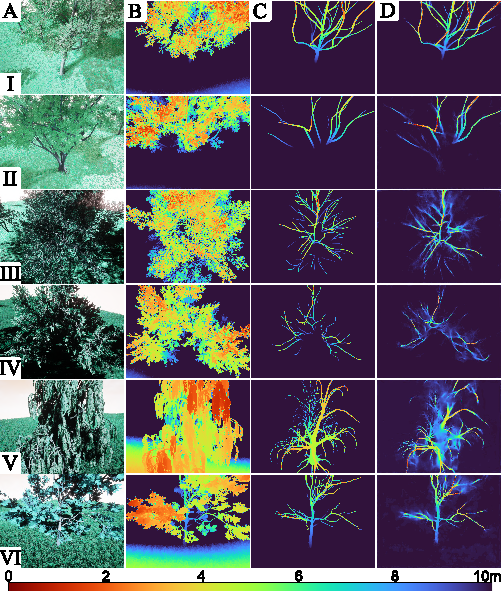
\includegraphics[width=1\columnwidth]{chapters/papers/OBR/figures/fig-4-qualitative-sim/fig-4-qualitative-sim-v05.pdf}
    \vspace{\figurevspaceabove}
    \caption{Simulation inputs and outputs from the test dataset. Input RGB image (A), input depth image (B), with the target ground truth depth \mbox{mask (C)} and predicted depth masks of TransUNet (D). Tree species are Elm (I), Amur Cork (II),  Black Alder (III), London Plane (IV), Weeping Beech (V), and American Sycamore (VI). Bottom colorbar denotes depth scale in meters.}
    \label{fig-4-qualitative-sim}
    \vspace{\figurevspacebelow}
    % \vspace{-0.2cm}
\end{figure}


Figure~\ref{fig-4-qualitative-sim} visualizes RGB and depth input data from simulated images of different trees, with the target ground truth depth map and the model prediction  of the best performing TransUNet. While the depth predictions of sparse trees appear very sharp, occluded branches due to foliage lead to blurrier depth maps. Nonetheless, the model is able to recover branch locations which are not easily inferable for humans or heuristic-based algorithms. The supplementary video contains a panning side-view of the resulting point-cloud from the depth maps.
%Qualitatively, the network outputs look quite similar on the simulation data, hence only the best performing TransUNet is shown.
%Since the networks show comparable average numerical performance, quantitative visualizations also look similar. Figure~\ref{fig-4-qualitative-sim} shows the output of TransUNet.


\subsection{Network Comparison} 
    %inference times, model complexity
    % Table: inference times and model complexities \\
    % - esanet fastest inference time, baseline and unet-regression have smallest number of parameters

%#########################################################################
Since onboard computational hardware on a UAV is restricted, the evaluation times of the network forward pass are of great interest. To estimate the model-specific inference times, the execution time of the forward pass on the test dataset for each model was measured when predicting a single image frame, repeated 15 times. The evaluation times were measured on server-mounted Nvidia Titan X GPUs. While this differs from onboard hardware performance, the relative difference between the networks will remain comparable. To measure time complexity, GFLOPs (Giga Floating-Point Operations per second), the number of multiply-accumulates to compute the model prediction on a single image, are exploited.

% \begin{figure}[!t]
%     \centering
%     \includegraphics[width=0.48\textwidth]{figures/timetable.pdf}
%     \vspace{\figurevspaceabove}
%     \caption{Inference times of the forward pass of the different models (15 runs of 5000 samples per model)}
%     \label{fig:inference_times}
%     \vspace{\figurevspacebelow}
% \end{figure}

% \begin{figure}
% \centering
% \begin{minipage}{.25\textwidth}
%   \centering
%     \includegraphics[1.0\textwidth]{figures/timetable.pdf}
%     \caption{Inference times of the forward pass of the different models (15 runs of 5000 samples per model)}
%     \label{fig:inference_times}
% \end{minipage}%
% \begin{minipage}{.25\textwidth}
% % \begin{table}[ht]
% \caption{Comparisons of model size and complexity}
% \label{tab:model_complexity}
% \centering
% \begin{tabular}{lll}
% \hline
% Model     & GFLOPs & Param. (M)  \\
% \hline \hline
% Baseline  & 256.7            & 31.04                  \\\hline
% U-Net     & 256.7            & 31.04                  \\\hline
% TransUNet & 204.68           & 88.92                    \\\hline
% ESANet    & \textbf{50.51}           & 46.91   
% \\\hline
% \end{tabular}
% % \end{table} 
% \end{minipage}
% \end{figure}
% \subsection{Model Complexity}
Table~\ref{tab:model_complexity} shows the results of the 15 evaluations on the test set comprising 7K images. One can observe that the ESANet performs significantly better in GFLOPs, with an 80\% decrease from baseline and U-Net. The space complexity, represented by the number of parameters (in millions), are roughly the same for all models (31M to 47M), except the TransUNet (89M) which has more than double the number of parameters due to the additional transformer layers. The last row reports the inference times in seconds for 15 frames. The fastest forward pass is achieved by the ESANet, in accordance with the GFLOPs analysis of the first row. Note that the baseline inference time includes the additional temporal overhead of masking the input sensor depth against the output binary segmentation, to create a depth map for comparison against the other regression networks.

% \begin{table}[ht]
% \caption{Comparisons of model size and complexity}
% \label{tab:model_complexity}
% \centering
% \begin{tabular}{lll}
% \hline
% Model     & GFLOPs & Param. (M)  \\
% \hline \hline
% Baseline  & 256.7            & 31.04                  \\\hline
% U-Net     & 256.7            & 31.04                  \\\hline
% TransUNet & 204.68           & 88.92                    \\\hline
% ESANet    & \textbf{50.51}           & 46.91   
% \\\hline
% \end{tabular}
% \end{table} 
% \begin{table}[!t]
% \caption{Comparisons of model size and complexity}
% \label{tab:model_complexity}
% \centering
% \begin{tabular}{l|llll}
% \hline
% Model       & Baseline  & U-Net & TransUNet & ESANet \\
% \hline
% GFLOPs $\downarrow$     & 256.7     & 256.7 & 204.68    & \textbf{50.51}\\
% \hline
% Parameters (M) $\downarrow$ & \textbf{31.04}     & \textbf{31.04} & 88.92     & 46.91\\
% \hline
% Inference Time (s) $\downarrow$& 0.341   & 0.309 & 0.336  & \textbf{0.279}
% \\\hline
% \end{tabular}
% \vspace{0.4pt} %0.4
% \end{table} 
\begin{table}[!t]
\caption{Comparisons of model size and complexity}
\label{tab:model_complexity}
\centering
\begin{tabular}{l|llll}
\hline
Model       & Baseline  & U-Net & TransUNet & ESANet \\
\hline
GFLOPs $\downarrow$     & 256.7     & 256.7 & 204.7    & \textbf{50.5}\\
\hline
Parameters (M) $\downarrow$ & \textbf{31.04}     & \textbf{31.04} & 88.92     & 46.91\\
\hline
Inference Time (s) $\downarrow$& 0.341   & 0.309 & 0.336  & \textbf{0.279}
\\\hline
\end{tabular}
\vspace{0.4pt} %0.4
\end{table} 


\subsection{Ablation Study}
    % (maybe in appendix/supplementary materials)\\
    % Table: Comparison Different loss functions (MSE best)\\
    % Table: different number of transformer layers for transunet (only skeleteon, mention in text that for whole image, zero layers gives best for whole imaeg)\\
    % Table: difference using only RGD, D, or RGB-D (RGB-D is best) on unet\\
    % Plot of depth impedement
    

%####################################################

%{ \setlength{\tabcolsep}{4pt}
%\begin{table}[!t]
%\caption{Results U-Net on tree skeleton for different loss functions}
%\label{tab:res_losses_branch}
%\begin{tabular}{@{}llllll@{}}
%\toprule
%Loss & MSE \phantom{iiiiiii} & RMSE \phantom{iiii} & LogRMSE & AbsRelErr & SqRelErr \\ \hline \hline
%\multirow{2}{*}{MSE} & \textbf{0.01129} & \textbf{0.10626} & \textbf{0.14032} & \textbf{0.08446} & \textbf{0.01728} \\
%& \textbf{0\%} & \textbf{0\%} & \textbf{0\%} & \textbf{0\%} & \textbf{0\%} \\ \hline
%\multirow{2}{*}{SmL1} & 0.01258 & 0.11217 & 0.14805 & 0.08746 & 0.01953 \\
%& -11.43\% &-5.56\% &-5.51\% &-3.55\% &-13.02\%  \\ \hline
%\multirow{2}{*}{AdSmL1} & 0.03009 &0.17346	&0.22833	&0.15302	&0.05 \\
%&-166.52\% &-63.24\% &-62.72\% &-81.17\% &-189.35\%  \\ \hline
%\multirow{2}{*}{MSEmCE} & 0.01203	&0.10969	&0.14537	&0.0887	&0.01862 \\
%&-6.55\% &-3.23\% &-3.6\% &-5.02\% &-7.75\%  \\ \bottomrule
%\end{tabular}
%\end{table}
%}

% { \setlength{\tabcolsep}{4pt}
% \begin{table}[!t]
% \caption{Results U-Net on tree skeleton for different loss functions}
% \label{tab:res_losses_branch}
% \begin{tabular}{@{}l|lllll@{}}
% \toprule
% Loss  & MSE \phantom{iiiiiii} & RMSE \phantom{iiii} & LogRMSE & AbsRelErr & SqRelErr \\ \hline \hline
% \multirow{2}{*}{MSE} & \textbf{0.01129} & \textbf{0.10626} & \textbf{0.14032} & \textbf{0.08446} & \textbf{0.01728} \\
% &\phantom{iiii}- & \phantom{iiii}- &\phantom{iiii}- & \phantom{iiii}- & \phantom{iiii}- \\ \hline
% \multirow{2}{*}{SmL1} & 0.01258 & 0.11217 & 0.14805 & 0.08746 & 0.01953 \\
% & (+11\%) &(+6\%) &(+6\%) &(+4\%) &(+13\%)  \\ \hline
% \multirow{2}{*}{AdSmL1} & 0.03009 &0.17346	&0.22833	&0.15302	&0.05000 \\
% &(+167\%) &(+63\%) &(+63\%) &(+81\%) &(+189\%)  \\ \hline
% \multirow{2}{*}{MSEmCE} & 0.01203	&0.10969	&0.14537	&0.08870	&0.01862 \\
% &(+7\%) &(+3\%) &(+4\%) &(+5\%) &(+8\%)  \\ \bottomrule
% \end{tabular}
% \end{table}
% }
{ \setlength{\tabcolsep}{4pt}
\begin{table}[!t]
\caption{Results U-Net on tree skeleton for different loss functions}
\label{tab:res_losses_branch}
\begin{tabular}{@{}l|lllll@{}}
\toprule
Loss  & MSE \phantom{iiiiiii} & RMSE \phantom{iiii} & LogRMSE & AbsRelErr & SqRelErr \\ \hline \hline
\multirow{2}{*}{MSE} & \textbf{0.011} & \textbf{0.106} & \textbf{0.140} & \textbf{0.084} & \textbf{0.017} \\
&\phantom{iiii}- & \phantom{iiii}- &\phantom{iiii}- & \phantom{iiii}- & \phantom{iiii}- \\ \hline
\multirow{2}{*}{SmL1} & 0.013 & 0.112 & 0.148 & 0.087 & 0.019 \\
& (+11\%) &(+6\%) &(+6\%) &(+4\%) &(+13\%)  \\ \hline
\multirow{2}{*}{AdSmL1} & 0.030 & 0.173	&0.228	&0.153	&0.050 \\
&(+167\%) &(+63\%) &(+63\%) &(+81\%) &(+189\%)  \\ \hline
\multirow{2}{*}{MSEmCE} & 0.012	&0.109	&0.145	&0.089	& 0.019 \\
&(+7\%) &(+3\%) &(+4\%) &(+5\%) &(+8\%)  \\ \bottomrule
\end{tabular}
\end{table}
\vspace{\figurevspacebelow} \phantom{i}
}

For computational reasons, all ablation studies were performed on a reduced dataset containing 18K training samples and 4K samples in the validation and test split each. 

To determine suitable training loss functions, the U-Net architecture was trained as a representative model on the following loss functions: MSE loss (Eq.~\ref{eq:MSE}, a smooth version of the L1 loss called SmL1 (comparable with the Huber loss)% where $\beta$ is the threshold between the L1 and L2 loss:
% {\small
% \begin{align}
% \label{eq:SmL1}
% SmL1 = \frac{1}{mn}\sum_{i=1}^m\sum_{j=1}^n l_{ij}, \phantom{iiiiiiiiii}\\
%     \text{with } l_{ij} = 
%     \begin{cases}
%     0.5(p_{ij}-t{ij})^2/\beta, & \text{if } \lvert p_{ij} -t_{ij} \rvert <  \beta\\
%     \lvert p_{ij} - t_{ij} \rvert - 0.5 \cdot \beta, & \text{otherwise}
% \end{cases} \nonumber
% \end{align}
% }%
, an adaptive version of the aforementioned SmL1 loss called AdSmL1 (optimizes the threshold for switching between the L2 to the L1 loss), and a mixture of MSE and cross entropy MSEmCE (MSE for pixel-wise depth regression and cross entropy for segmentation of the binary masked ground truth and prediction). Table~\ref{tab:res_losses_branch} presents the branch specific metrics (see Section~\mbox{\ref{subsec:training}}) after training the U-Net model for 20 epochs with the different losses. For clearer comparisons between the losses, the outputs are first normalized to be between 0 and 1 from initial outputs in the range of 0 to 10m. The percentages beneath the absolute loss values are with respect to the MSE loss in the first row.

For all metrics considered in the study, training on MSE yields better results than any other loss function on the tree skeleton. Since the predictions on the wooden parts of the trees are the primary interest, MSE was opted for as the loss function for training the final architectures.  

% The performance of ESANet with a sigmoid activation function in the last layer improves by an order of magnitude, due to fewer outlier predictions, hence this is also used in the final version.

% { \setlength{\tabcolsep}{5pt}
% \begin{table}[!t]
% \caption{Results TransUNet on tree skeleton for different number of transformer layers}
% \label{tab:res_transformer_branch_abl}
% \begin{tabular}{@{}llllll@{}}
% \toprule
% Input & MSE \phantom{iiiii} & RMSE \phantom{ii} & LogRMSE & AbsRelErr & SqRelErr \\ \hline \hline
% \multirow{2}{*}{0 Layers} & 0.01433 & 0.11971 & 0.15974 & 0.09828 & 0.02294 \\
% & 0\% & 0\% & 0\% & 0\% & 0\% \\ \hline
% \multirow{2}{*}{6 Layers} & 0.01209 & 0.10997 & 0.14668 & 0.08679 & 0.01928 \\
% & 15.63\% & 8.14\% & 8.18\% & 11.69\% & 15.95\% \\ \hline
% \multirow{2}{*}{12 Layers} & 0.0124 & 0.11134 & 0.14871 & 0.08969 & 0.01985\\
% & 13.47\% & 6.99\% & 6.9\% & 8.74\% & 13.47\%  \\ \hline
% \multirow{2}{*}{24 Layers} & \textbf{0.01159} & \textbf{0.10768} & \textbf{0.14364} & \textbf{0.08456} & \textbf{0.01846} \\
% & \textbf{19.12\%} & \textbf{10.05\%} & \textbf{10.08\%} & \textbf{13.96\%} & \textbf{19.53\%}  \\ \bottomrule
% \end{tabular}
% \end{table}
% }

% Table~\ref{tab:res_transformer_branch_abl} shows the effect of different number of transformer layers in the TransUNet architecture. There is a notable increase in performance (up to 19.53\% in the squared relative error, 19.12\% for MSE) on the tree skeleton when adding more transformer layers. Interestingly, when evaluating the transformer layer study on the whole image - not just the tree skeleton - the version with no additional transformer layers performs best, while introducing transformer layers worsens performance. This might be due to the ease of predicting the background pixels - however, the tree pixels are our primary interest. Whereas 12 layers seem optimal for medical image segmentation \cite{chen2021transunet}, for tree branch detection 24 layers yields the best performance. In consequence of the greatly increased cost induced by more trainable parameters, just 12 layers were used in the final TransUNet.

%{ \setlength{\tabcolsep}{5pt}
%\begin{table}[!t]
%\caption{Results U-Net on tree skeleton for different inputs}
%\label{tab:res_inputs_branch}
%\begin{tabular}{@{}llllll@{}}
%\toprule
%Input \phantom{iiii} & MSE \phantom{iiiiii} & RMSE \phantom{iiii} & LogRMSE & AbsRelErr & SqRelErr \\ \hline \hline
%\multirow{2}{*}{RGB-D} & \textbf{0.01129} & \textbf{0.10626} & \textbf{0.14032} & \textbf{0.08446} & \textbf{0.01728} \\
%& \textbf{0\%} & \textbf{0\%} & \textbf{0\%} & \textbf{0\%} & \textbf{0\%} \\ \hline
%\multirow{2}{*}{RGB} & 0.02144 &0.14641 &0.19626 &0.12612 &0.02864 \\
%& -89.9\% &-37.78\% &-39.87\% &-49.33\% &-65.74\% \\ \hline
%\multirow{2}{*}{D} & 0.01413 &0.11888 &0.15882 &0.10308 &0.02268\\
%&-25.16\% &-11.88\% &-13.18\% &-22.05\% &-31.25\%  \\  \bottomrule
%\end{tabular}
%\end{table}
%}


% { \setlength{\tabcolsep}{5pt}
% \begin{table}[!t]
% \caption{Results U-Net on tree skeleton for different model inputs}
% \label{tab:res_inputs_branch}
% \begin{tabular}{@{}l|lllll@{}}
% \toprule
% Input \phantom{iiii} & MSE \phantom{iiiiii} & RMSE \phantom{iiii} & LogRMSE & AbsRelErr & SqRelErr \\ \hline \hline
% \multirow{2}{*}{RGB-D} & \textbf{0.01129} & \textbf{0.10626} & \textbf{0.14032} & \textbf{0.08446} & \textbf{0.01728} \\
% &\phantom{iiii}- & \phantom{iiii}- &\phantom{iiii}- & \phantom{iiii}- & \phantom{iiii}- \\ \hline
% \multirow{2}{*}{RGB} & 0.02144 &0.14641 &0.19626 &0.12612 &0.02864 \\
% & (+90\%) &(+38\%) &(+40\%) &(+49\%) &(+66\%) \\ \hline
% \multirow{2}{*}{D} & 0.01413 &0.11888 &0.15882 &0.10308 &0.02268\\
% &(+25\%) &(+12\%) &(+13\%) &(+22\%) &(+31\%)  \\  \bottomrule
% \end{tabular}
% \end{table}
% }
{ \setlength{\tabcolsep}{5pt}
\begin{table}[!t]
\caption{Results U-Net on tree skeleton for different model inputs}
\label{tab:res_inputs_branch}
\begin{tabular}{@{}l|lllll@{}}
\toprule
Input \phantom{iiii} & MSE \phantom{iiiiii} & RMSE \phantom{iiii} & LogRMSE & AbsRelErr & SqRelErr \\ \hline \hline
\multirow{2}{*}{RGB-D} & \textbf{0.011} & \textbf{0.106} & \textbf{0.140} & \textbf{0.084} & \textbf{0.017} \\
&\phantom{iiii}- & \phantom{iiii}- &\phantom{iiii}- & \phantom{iiii}- & \phantom{iiii}- \\ \hline
\multirow{2}{*}{RGB} & 0.021 &0.146 &0.196 &0.126 &0.029 \\
& (+90\%) &(+38\%) &(+40\%) &(+49\%) &(+66\%) \\ \hline
\multirow{2}{*}{D} & 0.014 &0.119 &0.159 &0.103 &0.023\\
&(+25\%) &(+12\%) &(+13\%) &(+22\%) &(+31\%)  \\  \bottomrule
\end{tabular}
\end{table}
\vspace{\figurevspacebelow} \phantom{i}
}

To determine the importance of the contribution of the color and depth input respectively, the performance of the U-Net architecture trained on RGB-D images was compared with U-Nets trained on RGB images or depth (D) input only. The branch specific metrics of the U-Net model trained for 20 epochs on the different inputs is presented in Table~\ref{tab:res_inputs_branch}. 


\begin{figure}[!hpt]
    \centering
    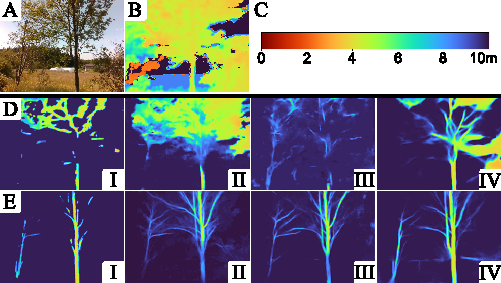
\includegraphics[width=\linewidth]{chapters/papers/OBR/figures/fig-6-qualtiative-real-comparison/fig-6-qualitative-real-comparison-half-v02.pdf}
    % \vspace{\figurevspaceabove}
    % \caption{Handpicked example outputs on two real-world images. Input RGB images (I-A, I-C), input depth images (I-B, I-D), and predicted network outputs: (II) Baseline, (III) U-Net, (IV) TransUNet, (V) ESANet. The network outputs in column A and C show the results on networks trained without domain transfer augmentation (II-A to V-A and II-C to V-C), and B and D with domain transfer augmentation (II-B to V-B and II-D to V-D).}
    \caption{Handpicked example output on a real-world images. (A) Input RGB image, (B) input depth images, (C) colormap for depth scale in meters, and predicted network outputs (D) without domain transfer augmentation and (E) with domain transfer augmentation: (I) Baseline, (II) U-Net, (III) TransUNet, (IV) ESANet.}
    \label{fig:real_world_data}
    % \vspace{\figurevspacebelow}
    \vspace{-0.2cm}
\end{figure}

In comparison to regular RGB color cameras, the additional depth information can provide vital information on the 3D structure of the tree, improving network performance.
Discarding the depth channel decreases performance by 38\% (RMSE) up to 90\% (MSE). On the other hand, dropping the three color channels leads to performance decreases of only 12\% (RMSE) up to 31\% (SqRelErr). Hence, the depth input alone is already sufficient to produce results close to the predictions based on RGB-D input images. We assume this to be due to the very accurate input depth images obtained in simulation, which contain most of the relevant information in high detail. As real depth sensors are not able to capture such high quality frames, the importance of RGB input images is expected to increase for real-world applications.
% \begin{figure}[!t]
%     \centering
%     \includegraphics[width=0.45\textwidth]{figures/d_quality_plot.pdf}
%     \vspace{\figurevspaceabove}
%     \caption{Performance of models trained on non-augmented data evaluated on test data with progressively stronger augmented depth input. Remark: the MSE for ESANet is discarded from the plot for depth impediment larger than $ 2 $ as it reaches values which are too high.}
%     \label{fig:d_robustness_ablation}
%     \vspace{\figurevspacebelow}
% \end{figure}

% Judging from the qualitative results in presented in Section~\ref{sec:real_world_results}
% % Figure~\ref{fig:real_world_data}, 
% it appears that the ESANet model generalizes better to real-world inputs than the remaining models. To verify this, network performance on progressively degraded inputs (Gaussian blur of increased kernel size and variance) was evaluated. The tests showed that U-Net and TransUNet degraded very similarly, however, the ESANet was less robust to changes in the depth input quality. This implies that the visually better performance of the ESANet model on real-world data in Figure~\ref{fig:real_world_data} is not due to  robustness towards degraded depth input, but rather because of better generalization capabilities as demonstrated in Table~\ref{tab:res_simulation_percent} for out-of-distribution data.

\vspace{-0.2em}
\subsection{Real-World Data} % esanet works best 
\label{sec:real_world_results}

\begin{figure*}[!hpt]
\centering
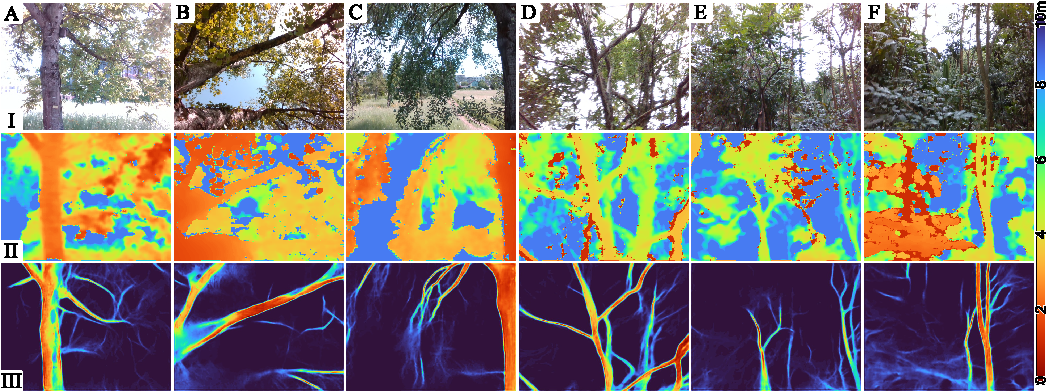
\includegraphics[width=\linewidth]{chapters/papers/OBR/figures/fig-5-qualitative-real/fig-5-qualitative-real.pdf}
% \vspace{\figurevspaceabove}
\caption{Qualitative real-world data of the ESANet on trees from Swiss temperate forests (A-C) and trees from a masoala rainforest (D-F). The network receives RGB (I) and depth (II) as input and computes the pixel-wise depth of the occluded branches (III). Colorbar on the right shows depth scale in meters.}
\label{fig-5-qualitative-real}
\vspace{\figurevspacebelow}
\end{figure*}


% GENERAL: Depth is cut-off at 10m, so far-away trees are labelled as background, even though they could be visible in the RGb image

%##################################################################################################

We provide a preliminary, qualitative, demonstration on real vegetation to demonstrate the feasibility of the approach on real-world data. To capture real-world data, images were taken with an Intel RealSense D435 depth sensor at a resolution of 640x480 pixels. Figure~\ref{fig:real_world_data} shows predictions for all models, trained on simulated data with and without domain transfer data augmentation. This clearly shows the importance of domain adaptation, considering that all models improve when using the augmented rather than the raw simulated data for the network training. While also true for the baseline, it still struggles with occlusions and predicts discontinuous branches (see Figure~\ref{fig:real_world_data}E-I). Visually, the ESANet (VI) appears to be the most robust to the domain change, as its predictions are smoother and less noisy. This could be due to depth and color inputs being encoded separately, which detaches the two different modalities. The above strategy can be helpful since the depth data changes quite drastically for the real-world samples in contrast to the color information. 

Results of the ESANet, trained on the augmented simulation dataset, on tree images from Swiss temperate forests and the Masoala Rainforest are shown in Figure~\ref{fig-5-qualitative-real}. The supplementary video contains a panning side-view of the resulting point-cloud of Figures~ \ref{fig:real_world_data}, \ref{fig-5-qualitative-real}. Overall, the results show that it is possible to generalize to real-world samples and to predict feasible leafless depth maps of trees given RGB-D data, even under very significant changes in the domain from simulated training.

% <TOOD> include some ground-truth evaluations from garage, to have comparison 

\section{Conclusion}
This letter demonstrates prediction of pixel-wise depth maps of partially occluded tree structures, given \mbox{RGB-D} input images. The networks are trained and evaluated on an extensive simulation dataset, with data post-processing performed to aid with domain adaptation on real-world data. When qualitatively evaluated on real-world images of trees from Swiss temperate forests and trees from the Masoala Rainforest at Zoo Zurich, the networks produce visually meaningful output depth maps. While predicting feasible outputs regarding the location of branches, the networks still struggle with input data that is very different from the training data. 

Given that the models currently perform better on synthetic rather than real data, future work will focus on improving the real-world performance. One possible approach is using a more diverse dataset, such as including images from a wider range of distances, more varied tree species, increasing tree density to better reflect the natural clustering of trees, or incorporating unsupervised domain adaption techniques \cite{csurka2021unsupervised_domain_adaption_survey}.
%bromley1993siamese (citation removed for space)
To further improve depth predictions, one might potentially explore alternative loss functions such as topological losses \cite{topological_loss} to impose constraints on the structural meaningfulness of the output. Additionally, the solution can be made more robust by reading sequential frames and outputting continuous segmentations, thus reducing dependence on lighting irregularities in singular frames and smoothing discontinuities between captures.
%flickering/video 

Since the envisioned use-case is UAV navigation in forest environments with dense vegetation, a natural next step would be to deploy the trained models on a drone in an online scenario to investigate the feasibility of using such architectures for path planning and obstacle avoidance. Assuming accurate output, this approach could then also be used to generate 3D models of occluded tree skeletons, by capturing images from around the tree. Considering the limited on-board computing hardware, optimizing performance and making the networks more lightweight should also be investigated. Potential applications of the system include collision avoidance in precision agriculture by detecting occluded branches for harvesting, pruning, or sensing, as well as robot navigation for search and rescue in dense forest environments, or for sensor placement and environmental monitoring. 


%%%%%%%%%%%%%%%%%%%%%%%%%%%%%%%%%%%%%%%%%%%%%%%%%%%%%%%%%%%%%%%%%%%%%%%%%%%%%%%%

% \addtolength{\textheight}{-12cm}   % This command serves to balance the column lengths
%                                   % on the last page of the document manually. It shortens
%                                   % the textheight of the last page by a suitable amount.
%                                   % This command does not take effect until the next page
%                                   % so it should come on the page before the last. Make
%                                   % sure that you do not shorten the textheight too much.

% %%%%%%%%%%%%%%%%%%%%%%%%%%%%%%%%%%%%%%%%%%%%%%%%%%%%%%%%%%%%%%%%%%%%%%%%%%%%%%%%

% \section*{APPENDIX}

% Appendixes should appear before the acknowledgment.
% \vspace{-1em}
\section*{ACKNOWLEDGMENTS}

The authors would like to thank Prof. Ce Zhang for 
providing access to computing clusters and helpful feedback, Davide Mambelli for initial work on the project, and Zoo Zürich for access to the Masoala Hall for data capture.
